\section{Introduction}
\label{sec:introduction}

LLM agents are increasingly undertaking complex, long-horizon tasks across real-world environments~\citep{yao2023react,shinn2023reflexion,jimenez2024swebench,gu2024toolsandbox,zhou2024webarena}. As task horizons expand, evaluating only final output results becomes insufficient to identify agent deficiencies and diagnose failure modes, bringing trajectory-level evaluation to the forefront of agent research~\citep{qian2024agentprocessbench,shi2025earlyeval}.

\begin{figure*}[t]
\centering
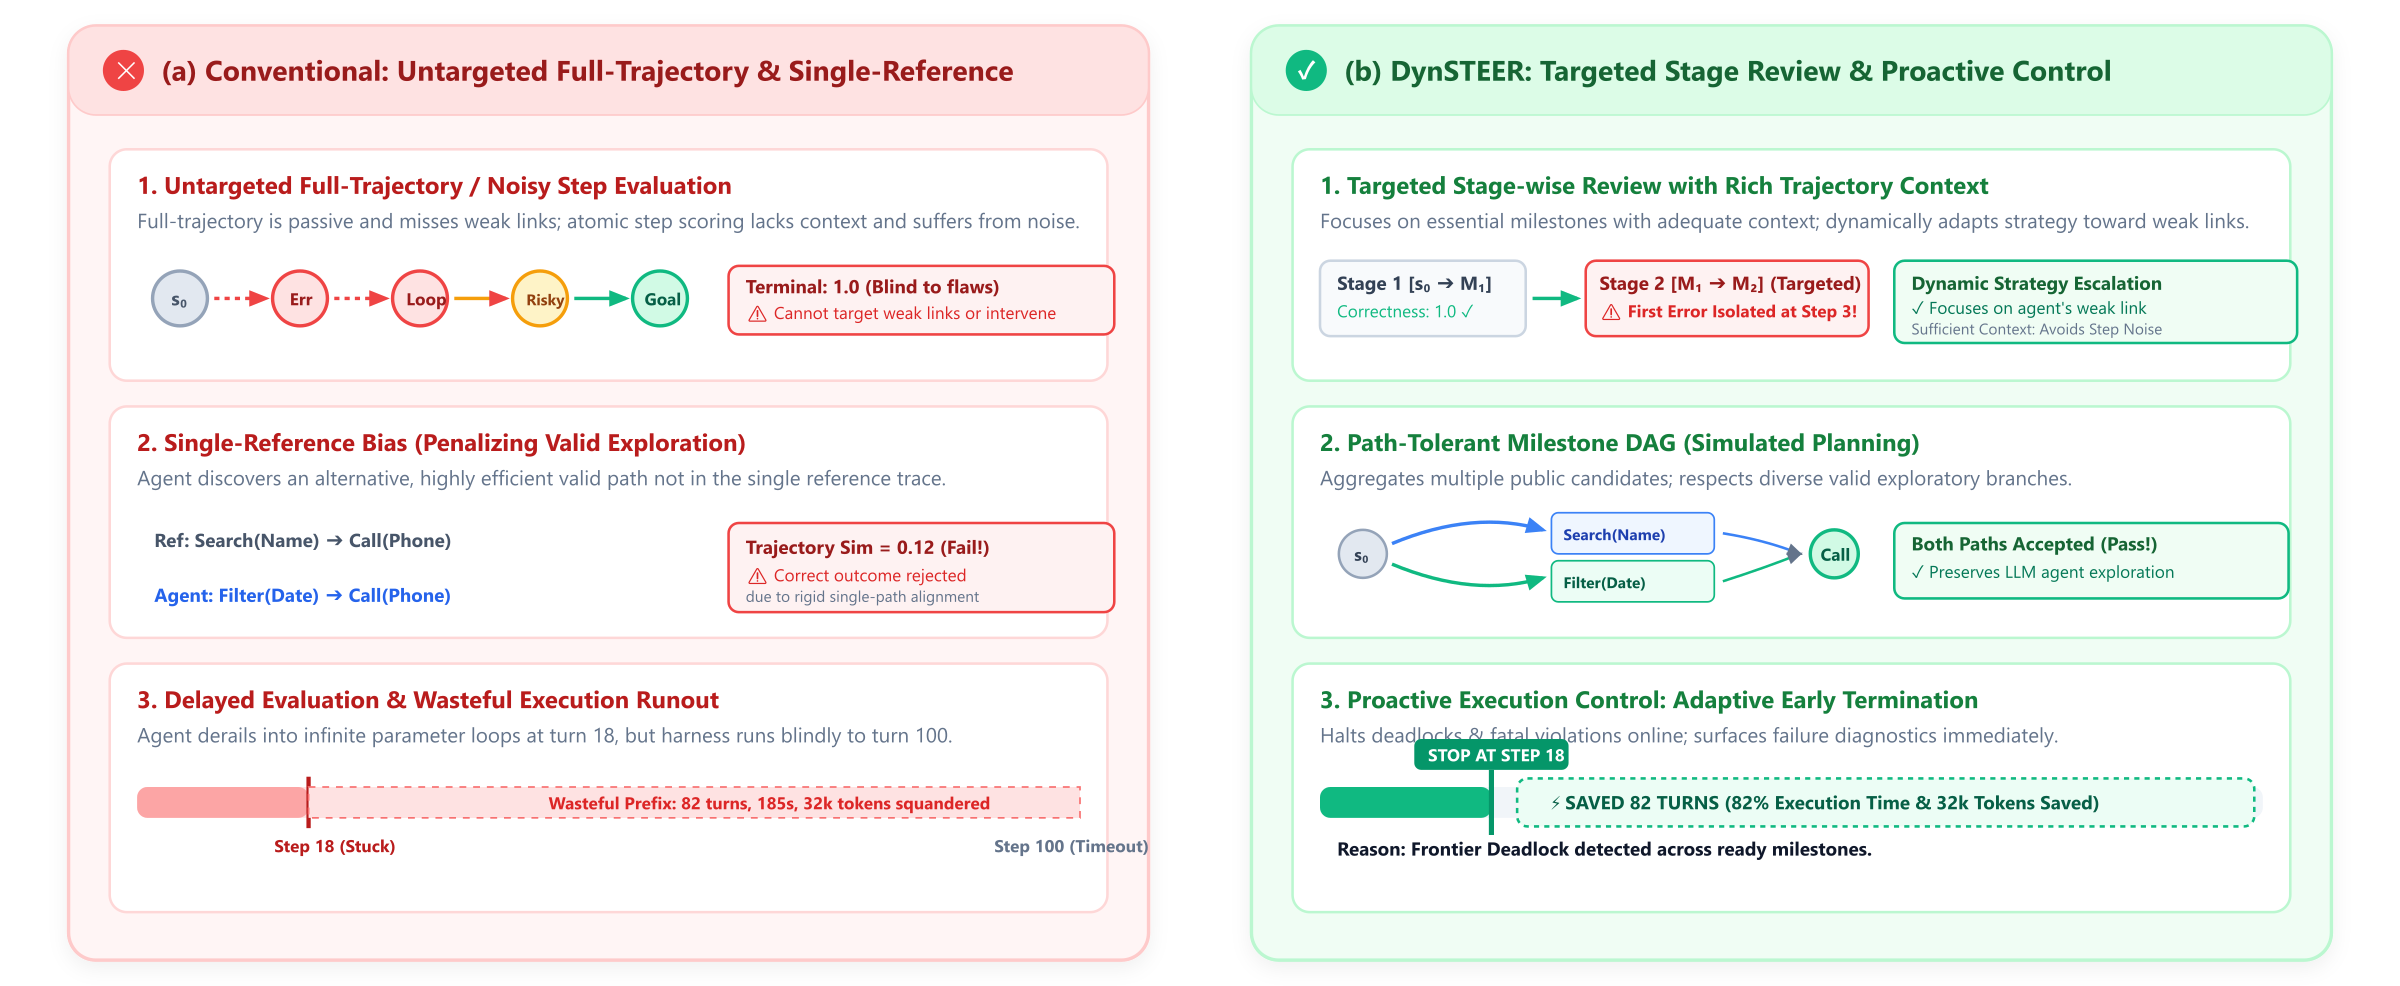
\includegraphics[width=0.96\textwidth]{figures/teaser_comparison.png}
\vspace{-0.25cm}
\caption{\textbf{Comparison of Agent Evaluation Paradigms.} (a) Conventional paradigms suffer from a lack of targeted stage context, single-reference bias, and wasteful delayed runouts. (b) \textsc{DynSTEER} enables targeted stage-wise evaluation with adequate context, accommodates diverse valid paths via milestone DAGs, and proactively halts deadlocks early, saving 34.51\% of wasteful steps.}
\label{fig:teaser_comparison}
\vspace{-0.35cm}
\end{figure*}

However, existing trajectory evaluation paradigms face three critical challenges: First, \textbf{Lack of Targeted Stage-wise Evaluation}: Whole-trajectory evaluation operates only post-hoc without dynamic intervention or adaptive strategies targeting an agent's truly weak segments, whereas atomic step evaluation lacks sufficient context and suffers from local noise, obscuring essential milestone progress; Second, \textbf{Single-Reference Trajectory Bias}: Existing evaluators typically measure similarity against a single reference trace, unfairly penalizing valid alternative strategies in open-ended tool environments; and Third, \textbf{High Cost and Delayed Feedback}: Evaluating full trajectories with heavy LLM judges incurs prohibitive latency and computational costs, while post-hoc evaluation fails to halt looping, hazardous, or hopeless executions early, causing severe resource waste.

To address these challenges, we introduce \textbf{DynSTEER}, short for \textbf{Dyn}amic \textbf{S}tage-wise \textbf{T}rajectory \textbf{E}valuation and \textbf{E}xecution-time \textbf{R}eview, a dynamic framework transforming agent evaluation into targeted, stage-wise execution review as illustrated in Figure~\ref{fig:teaser_comparison}b. First, to overcome untargeted full-trajectory and noisy step evaluations, DynSTEER segments rollouts into localized stages anchored by key completed actions and graph dominators, supplying adequate context to evaluate essential milestones and adaptively tune judging toward weak segments. Second, to eliminate single-reference bias, it compiles a path-tolerant milestone graph from public task views via multi-candidate simulated planning and majority consensus, capturing necessary task invariants to accommodate diverse legitimate exploration paths. Third, to curb evaluation costs and prevent runaway executions, it couples an uncertainty-adaptive multi-tier judge ladder with execution-time early stopping that intercepts fatal safety violations, structural failures, and progress deadlocks.

In summary, our contributions are as follows:
\begin{itemize}[leftmargin=*,itemsep=1.5pt,topsep=1pt]
    \item \textbf{Stage-wise Alignment and Targeted Process Evaluation:} We formulate a dominator-anchored stage alignment mechanism that isolates local evidence windows between completed milestones. This provides sufficient trajectory context to evaluate intermediate quality, covering correctness, efficiency, safety, and compliance, localizing first-error steps, and adaptively focusing on an agent's weak execution segments.
    \item \textbf{Path-Tolerant Task Blueprint Compilation:} We design an automated multi-candidate graph synthesis and strict-majority consensus pipeline that operates strictly over public task views. By compiling a milestone DAG with transitive reduction, our framework preserves topological flexibility and accommodates diverse valid exploration strategies without reference leakage.
    \item \textbf{Uncertainty-Adaptive Routing and Execution-Time Early Termination:} We establish a dynamic three-tier judge hierarchy that routes judging per dimension based on uncertainty, paired with active runtime interception of fatal minefields and progress deadlocks. In experiments, DynSTEER cuts wasteful execution steps on failed rollouts by 34.51\% and saves an average of 32.89s in net pipeline time per halted run.
\end{itemize}
